% !TeX TXS-program:compile = txs:///lualatex

\documentclass[a4paper,11pt]{article}
\usepackage[revgoku]{cp-base}
\graphicspath{{./graphics/}}
%variables
\donnees[%
	classe={1\up{ère} 2M2},matiere={[SPÉ.MATHS]},mois=Février,annee=2022,typedoc=CHAP,numdoc=8
]
%formatage
\author{Pierquet}
\title{\nomfichier}
\hypersetup{pdfauthor={Pierquet},pdftitle={\nomfichier},allbordercolors=white,pdfborder=0 0 0,pdfstartview=FitH}
%divers
\lhead{\entete{\matiere}}
\chead{\entete{\lycee}}
\rhead{\entete{\classe{} - \mois{} \annee}}
\lfoot{\pied{\matiere}}
\cfoot{\logolycee{}}
\rfoot{\pied{\numeropagetot}}

\begin{document}

\pagestyle{fancy}

\part{CH08 - Fonctions dérivées - Exercices}

\medskip

\begin{caide}
{\setlength\arrayrulewidth{1.5pt} \arrayrulecolor{titrebleu!35}
\begin{tabularx}{\linewidth}{Y|Y|Y|Y|Y|Y}
	\niveaudif{0}~~\textsf{Basique} & \niveaudif{1}~~\textsf{Modérée} & \niveaudif{2}~~\textsf{Élevée} & \niveaudif{3}~~\textsf{Très élevée} & \niveaudif{4}~~\textsf{Extrême} & \niveaudif{5}~~\textsf{Insensée} \\
\end{tabularx}}
\end{caide}

\exonum{0}

\medskip

On considère la fonction $f$ définie sur $\R$ par $f(x)=x^3+x^2+x+1$. On note $\mathscr{C}_f$ sa courbe représentative.

\begin{enumerate}
	\item Calculer $f(3)$.
	\item
	\begin{enumerate}
		\item Déterminer la dérivée $f'$ de la fonction $f$.
		\item En déduire la valeur de $f'(3)$.
		\item Déterminer une équation de $\mathscr{T}_3$, tangente à $\mathscr{C}_f$ au point d'abscisse 3.
	\end{enumerate}
	\item Déterminer une équation de $\mathscr{T}_{-1}$, tangente à $\mathscr{C}_f$ au point d'abscisse $-1$.
\end{enumerate}

\medskip

\exonum{1}

\begin{enumerate}
	\item Justifier le résultat obtenu sur les captures d'écran \ccalg{calculatrice} suivantes :
	\begin{center}
		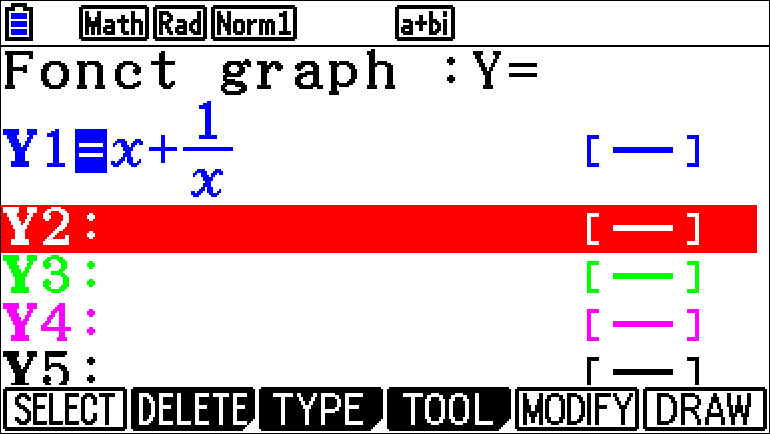
\includegraphics[height=2.5cm]{td04_exo01_a}~~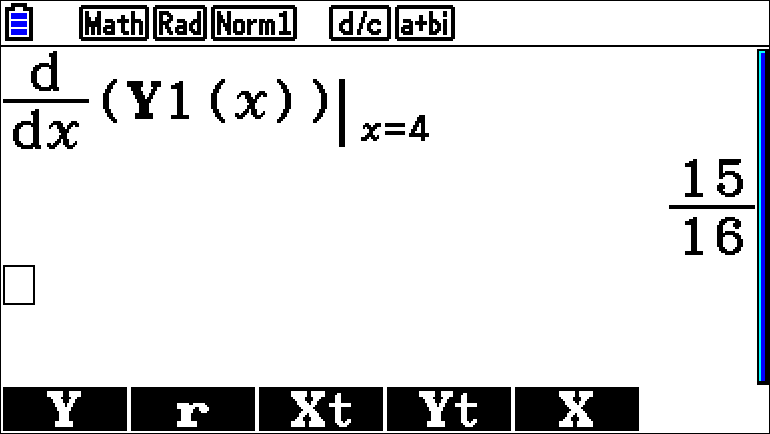
\includegraphics[height=2.5cm]{td04_exo01_b}
	\end{center}
	\item Justifier le résultat de la ligne \cxcas{L2} suivante :
	\begin{center}
		\begin{tikzpicture}[x=1cm,y=1cm,line width=1pt]
			\paramCF[larg=14,esplg=3pt,color=black,menu=true,titre=true,size=\small]
			\ligneCF[hc=0.66,hr=0.66]{$\mathsf{f(x):=10*sqrt(x)}$}{$\mathsf{x \mapsto 10\sqrt{x}}$}
			\ligneCF[hc=0.66,hr=0.66]{$\mathsf{f'(5)}$}{$\mathsf{2.23606797}$}
		\end{tikzpicture}
	\end{center}
\end{enumerate}

\medskip

\exonum{1}

\begin{enumerate}
	\item Déterminer la dérivée des fonctions suivantes, sans se soucier de l'ensemble de dérivabilité :
	\begin{enumerate}
		\item $f(x)=2x^3+4x^2-5x+6$ ;
		\item $g(x)=5x+\dfrac{2}{x}$ ;
		\item $h(x)=4\sqrt{x}-7x$.
	\end{enumerate}
	\item Déterminer une équation de :
	\begin{enumerate}
		\item $\mathscr{T}_2$, tangente à $\mathscr{C}_f$ au point d'abscisse 2 ;
		\item $\mathscr{T}_{-1}$, tangente à $\mathscr{C}_g$ au point d'abscisse $-1$ ;
		\item $\mathscr{T}_9$, tangente à $\mathscr{C}_h$ au point d'abscisse 9 ;
	\end{enumerate}
\end{enumerate}

\medskip

\exonum{2}

\medskip

Déterminer la dérivée des fonctions suivantes :

\begin{enumerate}
	\item $f(x)=\big(x^2+1\big) \times \big(-x^3+2x^2+5\big)$ définie et dérivable sur $\R$ ;
	\item $g(x)=(x+1)\sqrt{x}$ définie sur $\intervFO{0}{+\infty}$ et dérivable sur $\intervOO{0}{+\infty}$ ;
	
	\textit{\footnotesize \faHandPointRight[regular] \small on essayera de simplifier en mettant au même dénominateur\ldots}
	\item $h(x)=\dfrac{3x+1}{x-5} $ définie et dérivable sur $\R \backslash \left\lbrace \strut 5 \right\rbrace$ ;
	
	\textit{\footnotesize \faHandPointRight[regular] \small on essayera de simplifier le numérateur\ldots}
	\item $k(x)=2x+\dfrac{1}{x^2+1}$ définie et dérivable sur $\R$.
	
	\textit{\footnotesize \faHandPointRight[regular] \small on essayera de simplifier en mettant au même dénominateur\ldots}
\end{enumerate}

\medskip

\exonum{3}

\medskip

En utilisant les formules de \og dérivation composée \fg, déterminer la dérivée des fonctions suivantes :
\begin{enumerate}
	\item $f(x)=(3x+1)^3$ définie et dérivable sur $\R$ ;
	\item $g(x)=\sqrt{2x+1}$ définie sur $\intervFO{-\tfrac{1}{2}}{+\infty}$ et dérivable sur $\intervOO{-\tfrac{1}{2}}{+\infty}$ ;
	\item $h(x)=\sqrt{x-2}\,\big(x^2-1\big)$ définie sur $\intervFO{2}{+\infty}$ et dérivable sur $\intervOO{2}{+\infty}$ .
\end{enumerate}

\medskip

\exonum{2}

\medskip

On considère la fonction $f$ définie sur $\intervFF{0}{7}$ par $f(x)=x^3-11x^2+39x-20$.

\begin{enumerate}
	\item Déterminer, pour tout $x$ de $\intervFF{0}{7}$, l'expression de $f'(x)$.
	\item Étudier le signe de $f'(x)$ sur $\intervFF{0}{7}$.
	\item Déterminer le sens de variation de $f$ sur $\intervFF{0}{7}$.
\end{enumerate}

\medskip

\exonum{3}

\medskip

On considère la fonction $f$ définie par $f(x)=\dfrac{2x+1}{4x^2+4x+5}$. On note $\mathscr{C}_f$ sa courbe représentative.

\begin{enumerate}
	\item En travaillant sur le dénominateur de $f$, démontrer que $f$ est définie sur $\R$.
	\item Vérifier que, pour tout réel $x$, on a $f'(x)=\dfrac{-8x^2-8x+6}{\big(4x^2+4x+5\big)^2}$.
	\item Étudier, dans un tableau, le signe de $f'(x)$.
	\item Déterminer le sens de variation de $f$ sur $\R$.
	\item Parmi les trois courbes suivantes, laquelle pourrait être -- sans utiliser de calculatrice -- $\mathscr{C}_f$ ? Justifier.
	\begin{center}
		\tunits{0.8}{8}
		\tdefgrille{-3}{3}{1}{0.5}{-0.301}{0.3}{0.1}{0.05}
		\begin{tikzpicture}[x=\xunit cm,y=\yunit cm]
			\tgrilles[line width=0.35pt,lightgray] ; \axestikz*[width=0.75pt] ;
			\axextikz[width=0.75pt,size=\scriptsize]{-3,-2,...,2} ; \axeytikz[width=0.75pt,size=\scriptsize]{-0.3,-0.2,-0.1,0,0.1,0.2} ;
			\draw[very thick,red,domain=\xmin:\xmax,samples=250] plot (\x,{(2*\x+1)/(4*\x*\x+4*\x+5)}) ;
		\end{tikzpicture}
		~~~~
		\begin{tikzpicture}[x=\xunit cm,y=\yunit cm]
			\tgrilles[line width=0.35pt,lightgray] ; \axestikz*[width=0.75pt] ;
			\axextikz[width=0.75pt,size=\scriptsize]{-3,-2,...,2} ; \axeytikz[width=0.75pt,size=\scriptsize]{-0.3,-0.2,-0.1,0,0.1,0.2} ;
			\draw[very thick,blue,domain=\xmin:\xmax,samples=250] plot (\x,{-(2*\x+1)/(4*\x*\x+4*\x+5)}) ;
		\end{tikzpicture}
		~~~~
		\tdefgrille{-4}{2}{1}{0.5}{-0.301}{0.3}{0.1}{0.05}
		\begin{tikzpicture}[x=\xunit cm,y=\yunit cm]
			\tgrilles[line width=0.35pt,lightgray] ; \axestikz*[width=0.75pt] ;
			\axextikz[width=0.75pt,size=\scriptsize]{-4,-3,...,1} ; \axeytikz[width=0.75pt,size=\scriptsize]{-0.3,-0.2,-0.1,0,0.1,0.2} ;
			\draw[very thick,purple,domain=\xmin:\xmax,samples=250] plot (\x,{(2*(\x+1)+1)/(4*(\x+1)*(\x+1)+4*(\x+1)+5)}) ;
		\end{tikzpicture}
	\end{center}
\end{enumerate}

\end{document}